\documentclass{article}
\usepackage[utf8]{inputenc}
\usepackage[brazil]{babel}
\usepackage{fancyvrb}
\usepackage[alf]{abntex2cite}
\usepackage{graphicx}
\usepackage{hyperref}

\title{
  Participa.br: Uma plataforma de participação democrática do governo Brasileiro
}

\author{
  Joenio Costa\\
  \texttt{joenio@joenio.me}
  \and
  Mariel Zasso\\
  \texttt{mariel.zasso@gmail.com}
  \and
  Paulo Meirelles\\
  \texttt{paulormm@unb.br}
  \and
  Ricardo Poppi\\
  \texttt{ricabras@gmail.com}
}

\begin{document}

\maketitle

\section{Introdução}

% * Motivação (contexto da participação no governo Brasileiro antes do Participa.br)

A participação social no Brasil representa princípio jurídico-institucional
presente na Constituição Federal de 1988, que a definiu como forma de afirmação
da democracia e da consolidação da cidadania. 

Ao incorporar esse princípio como referência para a gestão pública, o Governo
Federal aprimora os processos de interação do Estado com a Sociedade e cria as
condições institucionais para a prática da democracia participativa. 

Com isso, verifica-se que, além da crescente participação social nas decisões
governamentais, as políticas públicas ganham maior legitimidade, uma vez que
expressam as atuais condições socioeconômicas e culturais da população
brasileira em suas diferentes realidades regionais.

Na estrutura administrativa do Poder Executivo Federal, cabe à Secretaria-Geral
da Presidência da República (SG/PR) a função de intermediar as relações do
Governo com as entidades da sociedade civil, conforme competências definidas
pela Lei 10.683/2003 e pelo Decreto no. 7.688/2012. Assim, a SG/PR é órgão
incumbido de assessorar diretamente a Presidenta da República e os órgãos e
entidades do Governo Federal no relacionamento e na articulação com os
movimentos sociais, o que inclui a criação e a implementação de canais que
assegurem a consulta e a participação popular na discussão e na definição da
agenda prioritária do país.

O Brasil tem um rico histórico de efetivação da democracia participativa, sendo
reconhecido mundialmente. Os instrumentos institucionalizados como conselhos de
políticas públicas e conferências nacionais foram profundamente ampliados na
última década, contando com um legado volumoso de práticas e realizações. 

A maioria dos programas de governo já conta com participação social prevista em
pelo menos uma de suas etapas. As práticas trazidas pelas novas mídias e pela
cultura digital podem interagir nesses espaços fortalecendo, ampliando e
aprofundando a democracia participativa, especialmente neste novo século,
quando consideramos o contexto das redes sociais digitais.

\section{Plataformas digitais de participação}

% * Fundamentação (referências sobre governo aberto, ferramentas de participação digital, noosfero, etc)

A nossa sociedade passa por grandes transformações, especialmente na maneira
como lida com a informação disponível. O avanço da cobertura da Internet e das
redes sociais e a apropriação desses novos meios de comunicação pelas novas
gerações transformou as práticas comunicacionais e afetou diversos setores da
sociedade, inclusive a Política e os Governos. Essa profunda transformação
permitiu que a a informação fluísse de maneria rápida e direta para além dos
meios e intermediários tradicionais, dependendo cada vez menos dos meios de
comunicação de massa. 

Nos últimos anos, observou-se a popularização de ambientes e ferramentas que
digitalizam e amplificam as redes de colaboração e amizade, e permitem
publicação fácil e instantânea, a exemplo dos assim chamados blogs e serviços
de redes sociais. Esses ambientes, com grande adesão no Brasil, permitem a
mobilização e a rápida disseminação de conteúdos,  e possuem um grande alcance
pois trafegam por extensas redes de contatos. Percebendo as oportunidades desse
novo canal de interação, diversas empresas buscam acompanhar o comportamento
desses novos e potenciais clientes para estabelecer contato direto com esses
novos atores sociais nas redes.

A rapidez desse novo canal de interação permite que as solicitações e
reclamações postadas via redes sociais (e os diálogos subsequentes) sejam muito
mais rápidas do que as enviadas pelo antigos canais de interação, como correio,
por exemplo. O acompanhamento e sistematização de todas as demandas dos
clientes também ficou muito mais fácil e rápido. Com menos agilidade para se
apropriar e acompanhar essas mudanças, os Governos também tem feito algumas
incursões nesse novo meio, como criando canais oficiais para novas demandas,
propondo consultas públicas em metodologias abertas ou até propondo a
construção de uma constituição pela rede, com no caso recente da Islândia.

%Desta forma, antes da existência do Portal Federal de Participação Social, a
%Secretaria Geral da Presidência da República utilizava prioritariamente a
%interação presencial, com o uso mínimo de interação via Internet para dialogar
%com a Sociedade ou realizar debates e ações que envolvessem os mecanismos
%formais de participação social instituídos pelo Decreto Presidencial nº
%8.243/2014 (Decreto que institui a Política Nacional de Participação Social -
%PNPS).

\section{O Participa.br}

%Desde outubro de 2011, a partir de uma oficina no seminário nacional de
%participação social, a Plataforma Federal de Participação Social (participa.br)
%começou a ser concebida conceitualmente.  No começo de 2013 uma versão teste da
%plataforma foi iniciada, e foi considerada a necessidade de envolver todos os
%cidadãos (especialmente aqueles que nas manifestações de junho de 2013
%demonstraram não se sentir representados pelo atual sistema político e que
%utilizaram as rede socias para se mobilizar e expressar o desejo de diálogo,
%incidência e representação sobre as decisões do poder público e suas políticas
%públicas). O desenvolvimento da Plataforma Federal de Participação Social, a
%partir de junho de 2013, obteve a máxima centralidade política para buscar
%novas formas de diálogo com a Sociedade.
%
%Incentivando os atores a conectar perfis, blogs e demais instâncias de produção
%de conteúdo na rede, o Portal de Participação Social (participa.br) se
%estabeleceu como espaço de participação social na rede e lançou as bases para
%se constituir como um repositório integrador do conhecimento sobre participação
%social, antes bastante disperso na internet e nas instâncias governamentais. 

% * Apresentar e descrever a plataforma Participa.br

Seguindo esta tendência surge no Brasil o Participa.br, o Portal Federal de
Participação Social, mantido pela SGPR (Secretaria Geral da Presidência da
República) com especial atenção de setores de importância estratégica, como a
SNAS/SGPR (Secretaria Nacional de Articulação Social) e o Departamento de
Participação Social (DPS). Trata-se de um ambiente virtual de participação
social, ou seja, um mecanismo de interação social que utiliza tecnologias de
informação e de comunicação, em especial a internet, para promover o diálogo
entre a administração pública federal e a sociedade civil.

%O portal já acolheu diversos processos participativos desde o
%seu lançamento, facilitando e ampliando o dialogo entre o Governo (Gestores
%Públicos) e Sociedade (Cidadãos). 

O portal busca dar evidência às formas de participação existentes e previstas
no decreto da PNPS (Política Nacional de Participação Social) no sentido de
contextualizar, organizar e facilitar o acesso do cidadão às formas de incidir
nas diversas etapas das políticas públicas do governo brasileiro que estão
sendo debatidas em suas comunidades.

O Portal dispõe de ambientes interativos e participativos para consultas
públicas e etapas virtuais de conferência, transmissão interativa de eventos e
reuniões, tornando-se um repositório transparente e agregador do conhecimento
sobre participação social disperso na rede. O portal de participação social se
propõe como um espaço onde a sociedade dialoga com diferentes agentes de
governo, trazendo contribuições e colaboração nas diversas etapas das políticas
públicas.

A plataforma organiza seus debates em torno de comunidades temáticas criadas a
partir do interesse da sociedade ou governo. A gestão das comunidades é
conjunta. A construção de um processo participativo dentro de uma comunidade
ocorre no objeto ``trilha'' a qual permite estabelecer um caminho colaborativo de
participação com diversas etapas. Cada etapa está ligada a uma ferramenta
digital de participação.  

\begin{figure}[h]
  \center
  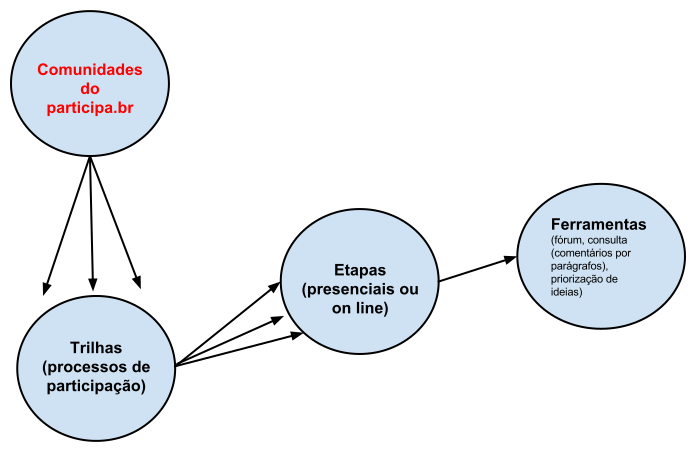
\includegraphics[scale=0.6]{imagens/diagrama-funcionamento.pdf}
  \caption{Diagrama de concepção de funcionamento do participa.br: comunidade possui trilhas; trilha possui etapas; etapa possui ferramenta.}
  \label{diagrama-funcionamento}
\end{figure}

Cada comunidade criada pode usufruir de uma ou mais trilhas de participação.
Cada trilha pode ter uma ou mais etapas participativas, presenciais ou online.
Cada etapa participativa possui uma ferramenta principal empregada no processo
que está sendo desenvolvido naquela etapa. As Comunidades são ambientes que
reúnem pessoas com interesses comuns. Facilitam a troca de ideias e a
interação, organizando os debates e aumentando o engajamento. 

O participa.br está descrito como um dos compromissos assumidos pelo Brasil no
Open Government Partnership (OGP) - Plano de Ação Brasileiro para a Parceria de
Governo Aberto.

A Plataforma Federal de Participação social pode ser acessada a partir do
endereço \url{http://www.participa.br}. A partir de uma interface clara, que permite
a navegação por temas, o Portal de Participação Social é um espaço onde os
diferentes agentes de governo, movimentos, organizações e cidadãos em geral
encontrarão solo fértil e facilitado para o exercício da construção
colaborativa de politícas publicas e diálogo sobre temas específicos, assim
como, para a pesquisa sobre participação social.

A capa do portal é composta por várias áreas (caixas ou box). Na parte superior
temos o cabeçalho de acordo com as normas da Secretaria de Comunicação da
Presidência da República. Logo abaixo está a barra de participação temática e
suas categorias para interação. Na sequência, temos a chamada para a
participação, proposição e mobilização. Outra preocupação da plataforma é dar
visibilidade aos processos internos de debate em uma área de destaque. O desejo
é dar ``destaque'' aos processos participativos mais quentes em discussão na
plataforma, ampliando as possibilidades de mobilização e engajamento do
cidadão.

As ferramentas participativas e suas metodologias também tem destaque na capa
do portal e é possível colocar qualquer processo participativo como chamada
principal, mediante necessidade. O bloco de notícias é operado pela equipe de
comunicação e redes sociais do portal que sempre acompanha e prioriza as
informações das comunidades temáticas.

O bloco de ``pessoas na rede'' permite que o cidadão acesse o perfil de outros
cidadãos e estabeleça o dialogo e o contato com outras pessoas interessadas em
debater determinados temas que ele tenha interesse. Em seu perfil pessoal o
cidadão tem ``vez e voz'' para expressar tudo o que deseja, sem nenhuma moderação
prévia. A moderação é posterior e só ocorre caso alguma proposição contrarie o
termo de uso do portal.

A equipe de comunicação acompanha/monitora as redes sociais e no bloco de
``redes sociais''  dá visibilidade às interações oriundas dos diversos perfis da
plataforma, assim como acompanha \texttt{\#hashtags} de interesse para a mobilização dos
diálogos e processos participativos nas redes sociais, como forma de atrair e
mobilizar o cidadão dessas redes para o diáogo e participação na construção de
políticas públicas na plataforma.

A capa contempla ainda núvem de TAGs, Comunidades de debate (comunidades na
rede, onde os processos participativos são realizados) e as principais trilhas
de participação (as que estão em destaque - mais quentes). O portal conta com
espaço de ajuda e indicação de como pode ser aproveitado.

\begin{figure}[h]
  \center
  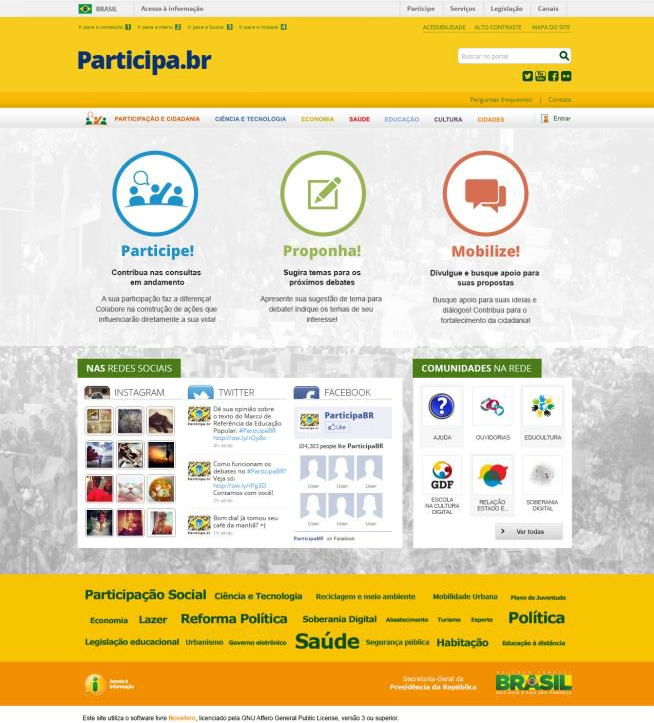
\includegraphics[scale=0.4]{imagens/screenshot-participa.png}
  \caption{Layout geral da capa do Participa.br com suas comunidades e participantes.}
  \label{screenshot-participa}
\end{figure}

Tendo por base a premissa de que a incursão e abertura de canais de acesso ao
poder público na rede aumentam o conhecimento das ações do governo e diminuem
as barreiras para participação de cidadãos, entidades e movimentos, o
Participa.br visa a construção de um conjunto de metodologias e ferramentas que
podem ser utilizadas por gestores e servidores para proporcionar novas formas
de participação social. Neste contexto é imprescindível mobilizar o cidadão
para que conheça e se aproprie dessas novas formas de participação.

Embora o Participa.br esteja sendo usado efetivamente pela Secretaria Geral
da Presidência da República desde junho de 2013, o seu lançamento oficial foi
feito pela Presidenta durante a Arena de Participação Social, de 22 a 24 de
maio de 2014 em Brasília/DF, junto com a assinatura do Decreto Presidencial nº
8243/2014 que institui a Política Nacional de Participação Social.

Durante o lançamento do portal foram exibidos dois vídeos que retratam a
retrospectiva de participação social no Brasil e os fundamentos básicos da
Plataforma Federal de Participação Social, assim como as falas no Ministro da
SG/PR e da Presidenta sobre a PNPS e o portal.

\begin{enumerate}
  \item Link do vídeo sobre o participa.br: \url{https://youtu.be/BRh2QLIu9yw}
  \item Fala do Ministro Gilberto Carvalho e da Presidenta da República sobre a PNPS e o participa.br: \url{https://youtu.be/Hj1xuqzHQT8}
\end{enumerate}

O Decreto Presidencial nº 8243/2014 que institui a Política Nacional de
Participação Social (PNPS) em seu Art. 6º inciso IX indica que: ``São instâncias
e mecanismos de participação social, sem prejuízo da criação e do
reconhecimento de outras formas de diálogo entre administração pública federal
e sociedade civil: ambiente virtual de participação social'' (GRIFO NOSSO).

Assim, alguns aspectos precisam ser observados na criação de ambientes virtuais
de participação social, especialmente para que tenhamos requisitos mínimos para
a plena participação social. Desta forma o Governo Federal, em todas as suas
instâncias, e especialmente Estados e Municípios, dentro do contexto maior do
Compromisso Nacional pela Participação Social (CNPS), deverão, de acordo
Decreto Presidencial nº 8243/2014, observar:

\begin{quote}
Art. 18.  Na criação de ambientes virtuais de participação social devem ser
observadas, no mínimo, as seguintes diretrizes:

\begin{enumerate}
  \item promoção da participação de forma direta da sociedade civil nos debates e decisões do governo;
  \item fornecimento às pessoas com deficiência de todas as informações destinadas ao público em geral em formatos acessíveis e tecnologias apropriadas aos diferentes tipos de deficiência;
  \item disponibilização de acesso aos termos de uso do ambiente no momento do cadastro;
  \item explicitação de objetivos, metodologias e produtos esperados;
  \item garantia da diversidade dos sujeitos participantes;
  \item definição de estratégias de comunicação e mobilização, e disponibilização de subsídios para o diálogo;
  \item utilização de ambientes e ferramentas de redes sociais, quando for o caso;
  \item priorização da exportação de dados em formatos abertos e legíveis por máquinas;
  \item sistematização e publicidade das contribuições recebidas;
  \item utilização prioritária de softwares e licenças livres como estratégia de estímulo à participação na construção das ferramentas tecnológicas de participação social; e
  \item fomento à integração com instâncias e mecanismos presenciais, como transmissão de debates e oferta de oportunidade para participação remota.
\end{enumerate}

\end{quote}

%Espera-se que, a partir da adesão de Estados e Município ao CNPS, a Plataforma
%Federal de Participação Social possa ser utilizada como ``Governo como
%Plataforma'' onde qualquer Estado ou Município poderá apropriar-se dela para
%realizar os seus processos participativos. Não obstante, 

Caso algum Estado ou Município não deseje utilizar a plataforma disponibilizada
pelo Governo Federal, este poderá instalar a sua própria instância do
Participa.br com todas as suas funcionalidades, pois este projeto utiliza
tecnologias livres e abertas, e todo o código do desenvolvimento está
disponível para qualquer cidadão. Poderão ainda customizar a plataforma de
acordo com o seu desejo, implementar melhorias, e fazer parte do consórcio de
desenvolvimento, maximizando ainda mais o reuso de código e recursos.

\section{Construção do Participa.br}

% * Planejamento do participa (reuniões iniciais, pessoas envolvidas na
%   concepção, planejamento, primeiros passos)
%
% * Relato da construção/implementação (ferramentas, software livre, noosfero,
%   consultores, produtos desenvolvidos, instituições envolvidas: Presidência,
%   UnB, etc, Ministérios, …, pessoas)
%
% * Casos de uso relevantes do Participa.br (plano de participação, arena net
%   mundial, etc…)

A ideia desta plataforma participativa surgiu em outubro de 2011, durante a
Oficina de Novas Mídias, Representação e Participação, desenvolvida no
Seminário Nacional de Participação Social. Naquela oportunidade foram
identificadas sugestões e propostas para o Portal. O resultado foi o primeiro
rascunho do projeto. Sua concepção, amadurecimento e desenvolvimento duraram
cerca de 1 ano e meio. O Portal entrou em funcionamento para sua primeira
consulta em julho de 2013.

A concepção do Portal de Participação Social também se inspirou em outras
iniciativas de participação ou redes sociais, tais como: 

\begin{enumerate}
  \item Participatório da Juventude da Secretaria Nacional da juventude\footnote{\url{http://juventude.gov.br}};
  \item Gabinete Digital do Governo do Rio Grande do Sul\footnote{\url{http://gabinetedigital.rs.gov.br}};
  \item Portal E-democracia da Câmara dos Deputados\footnote{\url{http://edemocracia.camara.leg.br}}.
\end{enumerate}

O Participa.br é uma ação de planejamento estratégico do Departamento de
Participação Social que integra a Secretaria Nacional de Articulação Social da
Secretaria Geral da Presidência da República. Dentro do contexto dos movimentos
e manifestações de junho de 2013 passou também a ser ação estratégica do
Gabinete Digital da Presidencia da República. Esse processo mobilizou os atores
internos da SG/PR para o desenvolvimento da plataforma como ação prioritária. O
portal passou a ser um novo canal de escuta e diálogo entre Governo e
Sociedade.

A própria construção e implantação do Portal de Participação Social se dá como
um processo de participação social, pois é feita de forma contínua,
participativa, colaborativa e integrada. 

A incorporação, no desenvolvimento do portal, da metodologia de desenvolvimento
oriunda dos projetos de Software Livre cumpre com os requisitos de
transparência, ao permitir o exercício de um processo de construção e
documentação em rede. 

Este processo permite que o cidadão ajude o Governo a construir as ferramentas
que irão contribuir com os processos de participação mediados por tecnologia.
Trata-se de um conceito de ``participação social no código fonte'' das
plataformas de software. Isso só é possível a partir do emprego de Software
Livre e licenças e tecnologias abertas. 

Durante o desenvolvimento da plataforma diversos atores foram envolvidos. A
sociedade participou de reuniões on line para levantamento de requisitos e
design participativo da plataforma. Na Secretaria Geral da Presidência também
foram realizadas reuniões de concepção e construção dos requisitos para o
desenvolvimento. A união de esforços e ideias resultou em uma sólida
conceituação e formulação do principais aspectos constitutivos do portal.

O processo de desenvolvimento também superou barreiras impostas pelo processo
tradicional de desenvolvimento de software na administração pública federal,
onde normalmente os softwares desenvolvidos, ainda que baseados em Software
Livre, não ficam acessíveis a Sociedade. Para unir esforços e ampliar o
aproveitamento de recursos, estabelecemos um consórcio de desenvolvimento que
uniu Sociedade e Governo, onde a premissa maior foi o retorno das melhorias
feitas no código fonte do software à arvore principal de desenvolvimento de sua
comunidade. A plataforma escolhida dentre várias estudadas foi o Noosfero\footnote{\url{http://noosfero.org}}.

De um lado, como sociedade civil, estavam a comunidade de desenvolvimento da
plataforma Noosfero e sua principal mantenedora de código fonte, a cooperativa Colivre\footnote{\url{http://colivre.coop.br}},
articulada com outros atores e comunidades de desenvolvimento da sociedade que
já utilizavam essa plataforma de rede social, tais como: Universidade de São
Paulo, Universidade de Brasília, e Cirandas.net (Iniciativa do Fórum Brasileiro
de Economia Solidária). Do outro, como Governo, estavam os atores
governamentais: Secretaria Geral da Presidência da República (SG/PR) por meio
da Secretaria Nacional de Articulação Social (SNAS), Secretaria Nacional da
Juventude (SNJ), Serviço Federal de Processamento de Dados (SERPRO), Ministério
do Planejamento, Orçamento e Gestão (MPOG) por meio da Secretaria de Lógistica
e Tecnologia da Informação (SLTI). A plataforma Noosfero é o ponto comum do
consórcio e todos os atores estão envolvidos em colaborar, melhorar suas
possibilidades e devolver as melhorias do software à Sociedade. São dois
conjuntos de atores que colaboram em pról do mesmo ponto comum de interseção: a
plataforma Noosfero. Desde o lançamento da plataforma novas ferramentas
continuam a ser desenvolvidas em conjunto, de forma colaborativa, transparente
e aberta, e novas metodologias de participação social mediadas por tecnologias
são incorporadas paulatinamente conforme a necessidade de cada ator do
consórcio.

A inspiração para criação da Plataforma Federal de Participação Social Participa.br foi
composta por várias vertentes. Uma delas foi o Participatório da Juventude.
Inicialmente o Participatório, a rede social para juventude da Secretaria
Nacional da Juventude, utilizou a ferramenta ELGG\footnote{\url{http://elgg.org}}. Uma rede social livre
desenvolvida em linguagem PHP. Após o lançamento, consolidação e resultados
positivos do Participa.br, empregando Noosfero em sua concepção, a Secretaria
Nacional da Juventude optou por adotar a mesma plataforma do Portal Federal da
Participação Social como forma de unir esforços e reduzir custos de
desenvolvimento e manutenção, passando a integrar também o consórcio de
desenvolvimento do Noosfero. 

O Portal do Software Público Brasileiro (SPB) do Ministério do Planejamento
também passou a integrar o consórcio de desenvolvimento colaborativo do
Participa.br a partir do momento em que também optaram por evoluir o SPB com a
adoção da plataforma Noosfero.

Alinhado a estes dois processos anteriores, o Serviço Federal de Processamento
de Dados (SERPRO), órgão responsável pela gestão de infraestrutura de sistemas
em produção do Governo Federal, também incorporou a tecnologia Noosfero em seu
ambiente interno. Trata-se do \texttt{\#você.serpro}, a rede social corporativa do
SERPRO. A partir dessa iniciativa de internalização dessa tecnologia o SERPRO
passou a oferecer essa plataforma como um dos produtos disponíveis para portal
de rede sociais no Governo Federal.

Todos esses processos de adoção e desenvolvimento colaborativo consolidam ainda
mais a comunidade de desenvolvimento em torno da plataforma Noosfero.

O ambiente de desenvolvimento do Participa.br é permeado e documentado por meio
de metodologias ágeis, utilizando-se de repositório público e sistema de
gerência de tarefas e bugs público através do serviço de gestão de projetos \url{Gitlab.com}. Todo o código é
licenciado em AGPLv3 ou licença compatível e está disponível para qualquer
cidadão.

\begin{figure}[h]
  \center
  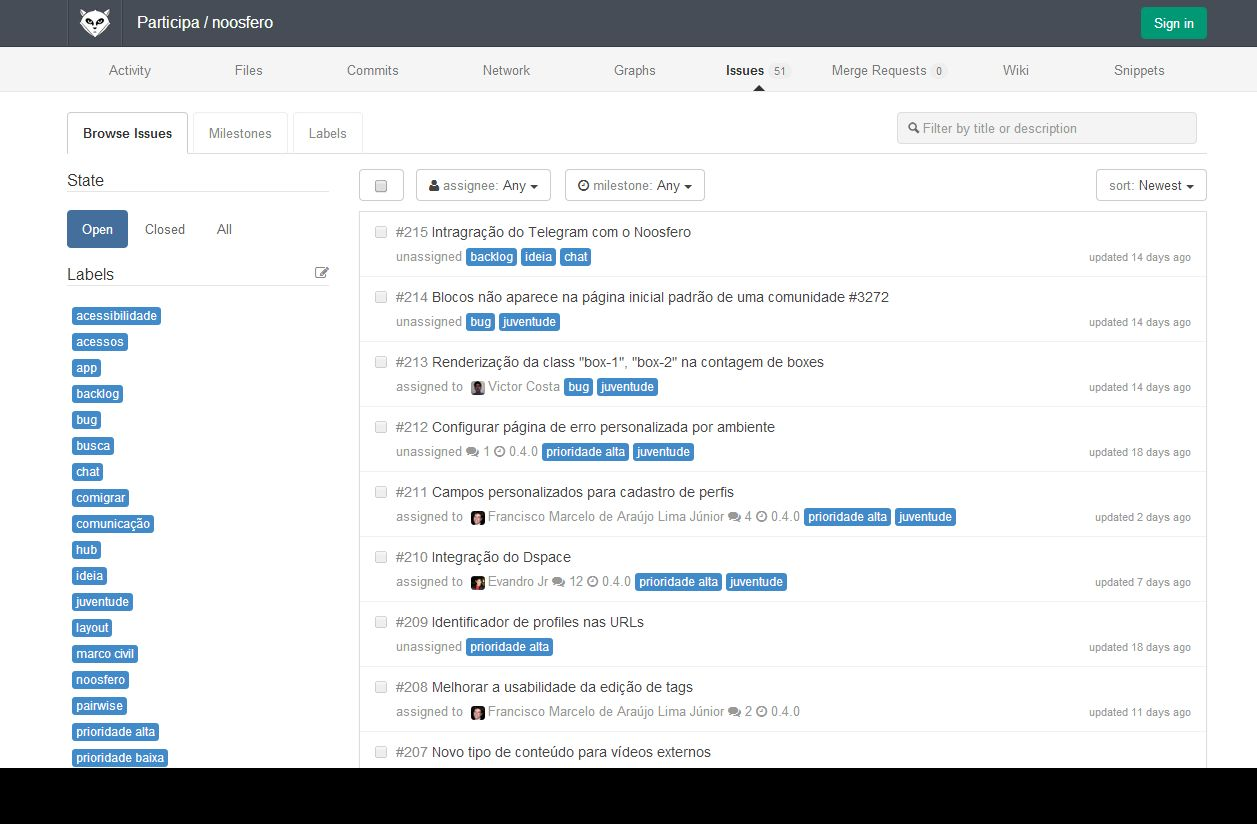
\includegraphics[scale=0.25]{imagens/screenshot-gitlab.png}
  \caption{Issues do sistema público de gerência de tarefas e bugs no Gitlab.com do Participa.br.}
  \label{screenshot-gitlab}
\end{figure}

Todo o processo de desenvolvimento da Plataforma Federal de Participação Social
(Participa.br) está alinhado aos objetivos da Política Nacional de Participação
Social (PNPS) descritos no Decreto Presidencial nº 8243/2014, onde é possível
destacar o objetivo VI que descreve: ``incentivar o uso e o desenvolvimento de
metodologias que incorporem múltiplas formas de expressão e linguagens de
participação social, por meio da internet, com a adoção de tecnologias livres
de comunicação e informação, especialmente, softwares e aplicações, tais como
códigos fonte livres e auditáveis, ou os disponíveis no Portal do Software
Público Brasileiro''.

Cabe ainda destacar que a consulta pública do Decreto Presidencial nº 8243/2014
que institui a PNPS também foi realizado por meio do Participa.br empregando um
processo participativo e colaborativo.

\subsection{Consultores do Participa.br}

A equipe de desenvolvimento do Participa.br contempla um conjunto de atores com
perfis diversificados. Cada um tem atuação em uma área relevante e específica,
mas seus esforços se somam ao contexto maior da equipe. As atividades envolvem
formulação de requisitos e diretrizes compreende gestão do desenvolvimento de
software, pesquisa e desenvolvimento metodológico, geração automatizada de
indicadores, dados linkados/web semântica, planejamento da comunicação e
monitoramento, capacitação para gestão de comunidades, planejamento e gestão de
trilhas de participação e realização de atividades presenciais de participação
com transmissão e interação online na plataforma. O link abaixo dá acesso ao
documento que detalha as atividades realizadas pelo time de consultores
integrantes da equipe de desenvolvimento  com o detalhamento de suas atividades
(produtos) realizadas na construção da plataforma.

\begin{description}
  \item [Documento de produtos dos consultores]
  \url{https://docs.google.com/document/d/1-eZO5KPiDy6SZXG6MazqCwU7geWkVlMklGR4EI9LgYQ/edit?usp=sharing}
\end{description}

Todo o processo de gestão e desenvolvimento das principais atividades que
conduziram a construção do Participa.br está descrito no quadro abaixo. São
atividades que envolveram reuniões, construção de artefatos, elaboração de
metodologias, implementações computacionais e outras ações. As atividades estão
dispostas cronologicamente e algumas possuem imagens ou links para melhor
exemplificar as ações.

\begin{description}

  \item [Outubro 2011] Oficina do portal da participação social no seminário
  nacional de participação social \footnote{\url{http://www.youtube.com/watch?v=IRE7Y0zWDsw}};
  Primeira notícia publicada na mídia (wireless mundi)
  \footnote{\url{http://www.wirelessmundi.inf.br/noticias-geral/161-governo-cria-portal-da-participacao-social}}

  \item [Novembro 2012]
  Formação da equipe do Participa.br.

  \item [Dezembro 2012]
  Escolha de ferramentas para a implementação do Participatório da Juventude da
  SNJ (Noosfero, ELGG e outras).

  \item [Janeiro 2013]
  A DITEC da SG/PR disponibiliza o ambiente com Noosfero
  <http://www.psocial.sg.gov.br/> para avaliação da equipe do Participa.br.

  \item [Abril 2013]
  Início do processo de seleção para contratação de consultores;
  Contratação do SERPRO para desenvolvimento e infraestrutura de hospedagem da plataforma Participa.br.

  \item [Maio 2013]
  Início do ciclo reuniões com a sociedade civil para a construção
  participativa e levantamento de requisitos e design da plataforma.

  \item [Julho 2013]
  Primeira consulta pública  no Participa.br para a construção colaborativa da
  Política Nacional da Participação Social (PNPS) e do Compromisso Nacional da
  Participação Social (CNPS).

  \item [Setembro 2013]
  Reunião sobre o que é o Participa.br e apresentação de ideias para a
  coordenação de comunicação do Portal.

  \item [Novembro 2013]
  Reunião de planejamento com ASCOM/SG-PR, Secretaria-Executiva/SG-PR e equipe Participa.br;
  Envio a sugestão de Plano de Comunicação para o Participa.br;
  Oficina com os consultores para aprender a usar o Noosfero;
  Primeiras sugestões de logo do Participa.br;
  Construção da lista de possíveis temas para comunidades do Participa.br. A meta era ter na plataforma temas essenciais para sociedade (Saúde, educação, mobilidade urbana, segurança e reforma política). Os temas foram os que mais apareceram nos protestos de junho de 2013. Infelizmente não foi possível abrigar debates com todos os temas, ou por falta de lideranças sociais dispostas a utilizar o Participa.br como plataforma de debate ou por falta de representantes do governo. A equipe do Participa.br continua empenhada neste sentido.;
  Continuação da oficina para aprender a usar o Noosfero;
  Início da mobilização para criação de comunidades. A equipe fez contato com diversos órgãos do Governo Federal e sociadade civil.

  \item [Dezembro 2013]
  Concurso Desafio de Ideias para a criação de aplicativos para o Participa.br (http://migre.me/l8smH);
  Criada a comunidade Ajuda no Participa.br para orientar os usuários sobre a utilização da plataforma;
  Reunião com represententes da CGU para a criação de comunidade. O órgão realizou consulta pública no Participa.br para a construção colaborativa  do Sistema Nacional de Ouvidorias ( www.participa.br/ouvidorias);
  Mudança na url do Participa.br;
  A equipe optou por não adotar o .gov.br, mas sim o .br. A intenção é deixar claro que não se trata de site do governo, mas sim de uma plataforma da qual a sociedade pode, e deve, se apropriar para debate e construção de políticas públicas;
  Criação da Comunidade de Educultura - do Departamento de Educação Popular;
  Mais tarde, foi realizada a consulta pública para a construção colaborativa da Política Nacional da Educação Popular (www.participa.br/educultura);
  Primeiras sugestões de tela para o Participa.br, que já estava em funcionamento, ou seja, algumas comunidades já realizavam processos participativos.

  \item [Janeiro 2014]
  Primeira reunião com equipe do Participatório da Juventude para integração dos sistemas;
  Ajustes e desenvolvimento de novas ferramentas para atendes às necessidades da comunidade Comigrar;
  Primeiras reuniões para o desenvolvimento de uma ontologia do Participa.br, com vistas à triplificação dos seus dados em RDF para disponibilização;

  \item [Fevereiro 2014]
  A equipe do Participa.br formulou documento contendo as principais funcionalidades da ferramenta para facilitar a apresentação aos órgãos de governo e sociedade;
  Também foi escrito um guia de estilo da plataforma (fonte, cores, etc);
  Início do planejamento para a realização da Arena Netmundial, que seria a maior consulta pública já realizada na internet;
  Estabelecimento de uma versão inicial da ontologia do particpa.br (OPA), para uso com a ontologia de participação social (OPS).

  \item [Março 2014]
  Foi realizado um hangout, com a participação remota de convidados, para lançar a consulta pública sobre governança da internet no Brasil: https://www.youtube.com/watch?v=tWbRQ125LW4;
  No dia 20 de março, as 17 horas, especialistas web, governo, blogueiros, jornalistas e internautas estarão ao vivo debatendo o futuro da governança da Internet. Quais direitos estão em jogo na sociedade conectada? Qual a importância da privacidade? A internet tem dono?;
  Venha conversar sobre essas e outras questões!;
  Primeiras experiências com streaming de estruturas sociais (meteor+d3 para visualizar formação de redes no Twitter);
  Comunidade Agroecologia realiza a Oficina do Ecoforte com transmissão online pelo Participa.br.

%No site www.participa.br você poderá interagir com:
%
% - Diogo de Sant´Ana, Secretario Executivo da Secretaria Geral da Presidência da República
%- Demi Getschko, Conselheiro do Comitê Gestor da Internet no Brasil (CGI.br), um dos responsáveis pela primeira conexão TCP/IP brasileira, em 1991. Por isso, é considerado um dos pais da Internet brasileira
%- Vírgilio Almeida, Coordenador do CGI.br. Atualmente é Secretário de Política de Informática do Ministério da Ciência, Tecnologia e Inovação - MCTI
%- Veridiana Alimonti, Membro do Comitê Gestor da Internet no Brasil (CGI.br) e advogada do Instituto Brasileiro de Defesa do Consumidor (Idec), com atuação na área de telecomunicações, incluindo as iniciativas relativas à governança da Internet e participação social na regulação dos serviços.
%
%Para participar você pode enviar perguntas e comentários através do Twitter e Facebook usando a hashtag #ArenaNetMundial. 
%
%O evento é parte das ações de mobilização do Arena NET mundial Participa.br e acontece durante a realização da consulta pública para saber o que a sociedade acha importante sobre o futuro da internet.

  \item [Abril 2014]
  A equipe planeja a cobertura colaborativa da Arena Netmundial. Pessoas de diversos estados desenvolveram na iniciativa. Além disso, estudantes puderam participar do evento como convidados pela SG-PR (foi a primeira vez que o Governo Federal articulou ação com IES neste sentido) -  http://migre.me/iMKQF;
  Desenvolvimento de aplicativo de participação social (HUB de Participação) para celular e tablet, empregado no Arena NET Mundial;
  ArenaNETmundial encerra com mais de 2 milhões de acessos na transmissão online;
  Divulgado o resultado da consulta pública sobre governança da internet:  "mais de 281 mil votos, recebendo quase trezentas propostas e aglutinando um total de 41 diretrizes para a elaboração de um novo modelo de governança global da internet, tudo definido de forma integralmente participativa";
  Durante o ArenaNETmundial, foram mantidos online  telões para visualização das redes sociais do Twitter confome relacionamento por retweet e vocabulário (observados somente tweets com hashtags de interesse). Estas redes eram também exibidas presencialmente no ArenaNETmundial;

  \item [Maio 2014]
  Maratona Hacker das organizações da sociedade civil. Promovida pela comunidade MROSC. no Participa.br
  http://www.brasil.gov.br/governo/2014/05/governo-promove-maratona-hacker-das-organizacoes-da-sociedade-civil ;
  Participa.br é apresentado durante o 15 Fórum Internacional Software Livre (FISL);
  Primeiras triplificações e disponibilização dos dados do participa.br em RDF via endpoint SparQL;
  Hangut com o ministro Gilberto Carvalho para conversar com a sociedade sobre participação social como método de governo
  http://gestao.participa.br/portal/blog/ministro-gilberto-carvalho-conversa-com-a-sociedade-sobre-participacao-social ;
  Acontece a Arena da Participação social onde a presidenta Dilma Rousseff lança oficialmente o Participa.br e sanciona o decreto n 8.243/14
  http://www.secretariageral.gov.br/noticias/2014/05/22-05-2014-abertura-da-arena-da-participacao-marca-a-conquista-dos-espacos-de-participacao ;
  Congelamento do Participa.br.

  \item [Julho 2014]
  Sistematizações para a Biblioteca Digital de gestão do conhecimento de participação;
  Análises iniciais dos dados do participa.br, disponibilizados via critérios semânticos em um endpoint SparQL e analisados em Python via mineração de redes e texto;

  \item [Agosto 2014]
  Versão inicial da API de recomendações para o participa.br: participantes, comunidades, trilhas e comentários recomendados para o participante, para comunidades ou para linha editorial.

\end{description}

\subsection{Recursos financeiros}

Os recursos financeiros empregados foram oriundos da Secretaria Geral da
Presidência da República. Dentro do contexto de desenvolvimento colaborativo e
em consorcio outros recursos foram disponibilizados por outros atores do
consórcio para desenvolver partes da ferramenta (plugins, funcionalidades e
metodologias). Por utilizar uma plataforma em Software Livre, o Participa.br
foi e continuará sendo beneficiado por todo desenvolvimento realizado no
Noosfero.

\begin{center}
    \begin{tabular}{ | l | l | l |}
    \hline
    Tipo de recurso   & Descrição & Valor em R\$ \\
    \hline
    Desenvolvimento   & 1.200 Pontos de Função         & 1.334.976,00 \\
    Consultoria       & recursos para 8 consultores    & 624.000,00   \\
    Viagens e eventos & diárias e passagens no projeto & 50.000,00    \\
    \hline
    TOTAL GERAL       &                                & 2.008.976,00 \\
    \hline
    \end{tabular}
\end{center}

\subsection{Recursos Humanos}

A composição da equipe do Participa.br está descrita abaixo e contempla os
atores diretamente envolvidos em seu de desenvolvimento e implementação.

\begin{description}

  \item [Ricardo Augusto Poppi Martins]
  - Coordenador Geral de Novas Mídias e outras Linguagens de Participação Social - Assessor da SG/PR.

  \item [Ronald Emerson Scherolt da Costa]
  - Coordenador da Equipe de Desenvolvimento do Participa.br - Assessor Técnico da SG/PR.

  \item [Daniela Soares Feitosa]
  - Consultora do participa.br e mestranda em Ciência da Computação pela Unniversidade Federal da Bahia. Integrante do time de desenvolvimento da plataforma Noosfero e sócia da Colivre.

  \item [Fabiano Rangel Cidade]
  - Consultor de Design Web e Arquiteto de Informação do projeto. Responsável pela coleta e análise de informações para definição de conceitos de criaçao e planejamento, gerando novas ideias, alternativas e conceitos gráficos que determinem as identidades visuais do projeto. Fundador e empresário de startup (faracy.com.br) segmento de Cultura Digital e cultura popular.

  \item [Joenio Marques da Costa]
  - Consultor do participa.br e mestrando em Ciência da Computação pela Universidade Federal da Bahia, membro do time de desenvolvimento da plataforma Noosfero, sócio-fundador da Colivre, administrador de sistemas com foco em tecnologias livres e contribuidor de projetos de software livre como Foswiki, Debian e Analizo.

  \item [Renato Fabbri]
  - Consultor do participa.br com ênfase em dados linkados, redes complexas e processamento de linguagem natural. Pesquisador, atualmente é candidato ao doutorando em física computacional no IFSC/USP. Participante co-fudador no labMacambira.sf.net, trabalhou com diversos grupos artísticos e de desenvolvimento tecnológico, com ênfase em cultura livre e digital.

  \item [Fernando Cruz]
  - Consultor do participa.br e Doutor em Ciência da Informação pela Universidade de Brasília e professor do curso de Engenharia de Software dessa mesma universidade. Trabalha com bibliotecas digitais, ontologias e web semântica.

  \item [Fabricio Solagna]
  - Consultor do participa.br e mestrando em Sociologia pela Universidade Federal do Rio Grande do Sul (UFRGS). É pesquisador e membro fundador do Grupo de Trabalho de Antropologia da Propriedade Intelectual (ANTROPI). É membro da Associação Software Livre.Org e organizador do Fórum Internacional de Software Livre (FISL). Foi coordenador-executivo do Gabinete Digital do Rio Grande do Sul de 2011 a 2013 (www.gabinetedigital.rs.gov.br). 

  \item [Ana Célia da Silva Costa]
  - Consultora do participa.br. Especialista em Marketing Digital pelo Instituto de Ensino Superior de Brasília. Formada em Comunicação com habilitação em Jornalismo, pela Universidade Federal do Amazonas. Pesquisadora de Social Media Monitoring. Trabalha na área desde 2005. Clientes: Embaixada do Reino Unido, Governo do Espírito Santo, Governo do Distrito Federal, Ministério da Saúde, Ministério da Integração, Governo da Bahia e outros. 

  \item [Grazielle Machado Fernandes]
  - Consultora do participa.br. Formada em jornalismo com especialização em política. Trabalha com comunicação e novas mídias desde 2008, ajudou a implementar a chamada assessoria 2.0 no ministério da Cultura e trabalhou em agência de públicidade como coordenadora de planejamento onde desenvolveu projetos para grandes clientes, entre eles: Partido dos Trabalhadores, Banco do Brasil, SESI, Unesco e BNDES. 

\end{description}

Além destes atores envolvidos diretamente no desenvolvimento e implementação do
Participa.br houve também enorme participação de comunidades de Software
Livre e algumas Entidades preocupadas com o tema do projeto.

\begin{itemize}

  \item Comunidade Noosfero
  \item Colivre - Cooperativa de Software Livre - Salvador - Bahia
  \item STOA/USP
  \item Comunidade UNB
  \item Grupo de alunos e professores de desenvolvimento do Laboratório LAPIS da UNB/Gama em Brasília
  \item SERPRO
  \item Secretaria Geral da Presidência (SG/PR)
  \item Ministério do Planejamento Orçamento e Gestão (MPOG)
  \item Portal do Software Público
  \item Secretaria de Logística e Tecnologia da Informação (SLTI)
  \item EITA (Cooperativa de Economia Solidária)
  \item Blogoosfero (Rede livre de blogs)

\end{itemize}

\subsection{Recursos tecnológicos}

O Noosfero é uma plataforma web livre para provedores autônomos de redes
sociais e sites 2.0, com características que permitem uma fácil adaptação do
sistema para as mais variadas necessidades de comunicação por meio da criação
de redes sociais, sites e blogs na Internet e intranet. Esta ferramenta se
adequa de modo sui generis a demanda de um portal de participação social, pois
além de ser um software livre, alinhado portanto com  a proposta de
participação social no código fonte, ele se mostra viável atendendo amplamente
as necessidades de uma rede social almejada pela Secretaria Geral da
Presidência da República.

Como essa plataforma é uma tecnologia aberta e disponível, uma organização pode
deixar de ser apenas ``usuária'' e passar a ser um provedor de uma rede social e
de sites 2.0, ao mesmo tempo.

O Noosfero teve seu lançamento oficial em 2009. Por conta da capacidade de
autonomia e liberdade tecnológica inerente a esse projeto, ele hoje é utilizado
com diferentes finalidades em diversos estados do Brasil, assim como em outros
países do mundo, como a Suíça, Alemanha e Japão.

O foco da plataforma Noosfero é ser uma rede social para produção e publicação
de conteúdo multimídia na Internet. Tudo o que for inserido na plataforma web
pode ser compartilhado de forma colaborativa. Ao fazer o cadastro, a/o
usuária/o internauta ganha um perfil, que pode também ter a função de site ou
blog, com sistema de notificação de comentários e adição de amigos.

Cada perfil de usuário funciona como uma página pessoal com o privilégio de
personalização de layout, como também do endereço de acesso (URL). O usuário
pode ainda utilizar o espaço para expor suas ideias, montar galerias de fotos e
vídeos, criar eventos (agenda), compartilhar interesses e preferências, além de
promover debates.

Isso significa que conteúdos diversos, como imagens, textos, documentos e
agenda de eventos podem ser inseridos de maneira descentralizada por pessoas
que não entendem nada de programação.

O processo de desenvolvimento de portais (ambiente online) com um mínimo de
complexidade é formado por dois elementos principais: a parte da frente
(conhecida no jargão técnico como {\it ``frontend''}) e os códigos que garantem o
funcionamento do ambiente e a comunicação com o banco de dados ({\it ``backend''}).

Do ponto de vista técnico, a plataforma Noosfero utiliza as seguintes
tecnologias livres:

\begin{description}

  \item [Banco de Dados PostgreSQL\footnote{\url{www.postgresql.org/about}}]

  Resultado de uma ampla evolução tecnológica que se iniciou na Universidade de
  Berkeley, Califórnia. Atualmente, esse sistema de banco de dados é utilizados
  por organizações que são referência no mundo como, por exemplo, The
  Washington Post U.S., Apple, Fujitsu, Skype, Departamento de Estado do
  Governo dos EUA, entre outras organizações internacionais.  No Brasil, existe
  uma forte comunidade de usuários (www.postgresql.org.br) que, por exemplo,
  organiza anualmente o PGBR: o maior evento sobre PostgreSQL das Américas
  \footnote{\url{http://pgbr.postgresql.org.br/2011/evento.php}}.

  \item [Linguagem de programação Ruby\footnote{\url{www.ruby-lang.org}}]

  Ruby é uma linguagem de programação interpretada multiparadigma, de tipagem
  dinâmica e forte, com gerenciamento de memória automático, originalmente
  planejada e desenvolvida no Japão em 1995, por Yukihiro "Matz" Matsumoto,
  para ser usada como linguagem de script. Ruby suporta programação funcional,
  orientada a objetos, imperativa e reflexiva. Ela é hoje bastante utilizada em
  plataformas web de alcance internacional como, por exemplo, Groupon,
  Mailee.me entre outras plataformas.

  \item [Framework de aplicações web Ruby on Rails]
  
  Ruby on Rails é um framework livre que amplia a velocidade e facilidade no
  desenvolvimento de sites orientados a banco de dados (database-driven web
  sites), uma vez que é possível criar aplicações com base em estruturas
  pré-definidas. As aplicações criadas utilizando o framework Rails são
  desenvolvidas com base no padrão de arquitetura MVC.

  \item [Servidor web Apache\footnote{\url{http://apache.org/}}]

  O servidor Apache é considerado o mais bem sucedido servidor web, pois numa
  pesquisa realizada em dezembro de 2007 pelo NetCraft, foi constatado que a
  utilização do Apache representa 47.20\% dos servidores ativos no mundo. Em
  maio de 2010, o Apache alcançou a marcar de servir de base para mais de  66%
  dos milhões de sites mais movimentados do mundo.
 
\end{description}

Todo o processo de desenvolvimento e hospedagem da plataforma em produção
está  baseado na estrutura do SERPRO que utiliza um servidor de 8gb de
memória, disco rígido (``HD'') de 82gb, processador Intel(R) Xeon(R) CPU E7-
4870 @ 2.40GHz com 8 cores.
 
\section{Resultados}

% * Legados (plataformas e ferramentas de software desenvolvidas, impacto em
%   outras iniciativas, projetos que nasceram inspirados no participa.br, pessoas
%   e grupos que tiveram formação em processos de participação por conta do
%   envolvimento no projeto, etc…)

Atualmente o Participa.br dispõe de mais de 24 comunidades temáticas. Cada
comunidade está construindo o seu caminho (trilha) e estabelecendo os seus
processos participativos (etapas e ferramentas). Algumas já possuem mais de uma
trilha de participação em funcionamento.

Dentre estas, há comunidades temáticas que se constituem como espaços para a
proposição e o debate de ideias que poderão se tornar políticas públicas. As
comunidades temáticas devem ser geridas por representantes do Governo e da
Sociedade Civil. Os órgãos de governo presentes, que participam de comunidades
temáticas, são: o  Ministério do Planejamento, Orçamento e Gestão (MPOG);
Ministério das Comunicações (MC); Universidade de Brasília (UnB); Serviço
Federal de Processamento de Dados (Serpro); Ministério da Justiça;
Secretaria-Geral da Presidência da República e Controladoria-Geral da União.
Algumas organizações da Sociedade Civil e Governos Estaduais também estão
presentes na plataforma: Associação Software Livre e Governo do Distrito
Federal.

Podemos destacar algumas das comunidades e processos participativos realizados
no Participa.br que obtiveram maior mobilização, interações e destaque:

\begin{description}

  \item [Política e Compromisso Nacional de Participação Social]

  Duas consultas públicas foram realizadas para que a Política Nacional de
  Participação Social (PNPS) e o Compromisso Nacional pela Participação Social
  (CNPS) tomassem forma. As duas iniciativas, foram elaboradas de maneira
  colaborativa, ou seja, a sociedade pôde participar de todo o processo
  comentando e acrescentando ideias durante as consultas públicas.

  Representantes da sociedade civil e integrantes da população tiveram a
  oportunidade de propor sugestões aos textos-base. Lançados pela
  Secretaria-Geral da Presidência da República, os dois textos normativos foram
  resultado da contribuição coletiva.

  A proposta do Compromisso Nacional pela Participação Social, como já
  explicitado, é reflexo dos debates entre os governos federal, estadual e
  municipal sobre a necessidade de reconhecer a participação social como
  estratégia para a democratização das decisões sobre políticas públicas. O
  objetivo é estabelecer diretrizes para a promoção da participação social como
  método de governo e para o fortalecimento dos mecanismos e instâncias de
  diálogo entre Estado e sociedade civil, com vistas à consolidação da
  democracia participativa no país.

  O Decreto Presidencial nº 8.423/2004, já mencionado, cria a Política Nacional
  de Participação Social (PNPS), visa fortalecer os mecanismos e as instâncias
  de participação social e diálogo entre o governo federal e a sociedade civil,
  estabelecendo os objetivos que afetam a gestão governamental como um todo e
  explicitar os princípios e diretrizes a serem observados pelos órgãos do
  governo federal.

  \item [Comigrar – 1ª Conferência Nacional sobre Migrações e Refúgio]

  A 1ª Comigrar foi coordenada pelo Ministério da Justiça, por meio da
  Secretaria Nacional de Justiça/Departamento de Estrangeiros-DEEST, em
  parceria com o Ministério do Trabalho e Emprego e o Ministério das Relações
  Exteriores, com o apoio da Organização Internacional para as Migrações-OIM e
  do Programa das Nações Unidas para o Desenvolvimento-PNUD. Seu objetivo foi
  reunir migrantes, profissionais envolvidos na temática migratória,
  estudiosos, servidores públicos, representações diversas que vivenciam a
  realidade da migração e do refúgio, para uma reflexão coletiva e elaboração
  de aportes para a construção da Política e do Plano Nacional de Migrações e
  Refúgio.

  O processo de implementação da 1ª Comigrar foi realizado por meio de eventos
  participativos de mobilização dos atores locais que trabalham e convivem com
  diferentes contextos da temática migratória. Esse processo participativo, por
  meio de conferências presenciais, virtuais e livres, teve início em 2013, e
  culminará na Etapa Nacional da Comigrar, a ser realizada em São Paulo, em
  2014. Na etapa virtual, os participantes apresentaram propostas à etapa
  nacional da Comigrar, no âmbito dos cinco eixos temáticos, independente de
  onde estejam no país ou no mundo. A Coordenação Executiva Nacional (CEN) fez
  a facilitação desta conferência virtual, no período de 10 de fevereiro e 23
  de março.

  Essa foi a primeira fase preparatória de uma Conferência brasileira realizada
  inteiramente em meio virtual, o que demonstra toda a potencialidade do Portal
  Participa.br.

  \item [Sistema de Ouvidorias]

  A ideia de criação do Sistema surgiu, ainda em 2012, a partir da visão de que
  o funcionamento integrado das ouvidorias do Poder Executivo Federal é
  essencial para garantir atendimento de excelência às manifestações dos
  cidadãos e o aprimoramento constante de políticas e de serviços públicos,
  tendo em vista o fortalecimento da participação social como meta e como
  método de realização do Estado Democrático de Direito.

  Uma das estratégias para a elaboração da proposta do Sistema de Ouvidorias
  foi a criação de um processo participativo. Na primeira etapa, foram
  coletados dados e informações a respeito das ouvidorias públicas brasileiras,
  bem como de institutos congêneres, a exemplo dos ombudsmen europeus. Na
  segunda etapa, houve a 3ª Reunião Geral de Ouvidorias Públicas, nos dias 21 e
  22 de março de 2013, para se realizar ao debate em torno da normatização do
  Sistema de Ouvidorias Públicas Federais. Entre os dias 16 de maio e 16 de
  julho de 2013, a sociedade pôde compartilhar ideias e enviar sugestões, por
  meio da Internet, para a redação final do Decreto que regulamenta o Sistema
  de Ouvidorias Públicas Federais. A Ouvidoria-Geral da União mediou a
  discussão, com a sugestão de tópicos, questões relevantes e, eventualmente,
  na formulação de novas propostas aos participantes. A nova minuta de Decreto
  levou em consideração as opiniões manifestadas durante a consulta. A consulta
  pública foi realizada pela Controladoria-Geral da União (CGU), em parceria
  com o Ministério da Justiça (MJ).

  Em 2014, nova trilha foi criada com a finalidade de estabelecer os princípios
  que devem orientar a elaboração de uma lei a respeito das Ouvidorias.

  \item [Participação, Planejamento e Orçamento]

  A Comunidade é um espaço de diálogo e colaboração da comunidade de
  participação no planejamento e orçamento do governo federal. Seus integrantes
  tiveram a oportunidade de sugerir os Projetos de Lei de Diretrizes
  Orçamentárias nos anos de 2014 e 2015, processo de consulta à sociedade
  elaboração do PLDO conta com um. 
Entre 2012 e 2013 a discussão para LOA envolveu cerca de 270 pessoas, entre representantes de entidades formais (sindicatos, conselhos, ONGs) e cidadãos não organizados, interessados em discussões setoriais envolvidas no processo orçamentário.

  \item [Parceria Governo Aberto]

  A primeira consulta realizada por essa comunidade foi a proposta de portaria
  que estabelece o Grupo de Trabalho da Sociedade Civil para a Parceria Governo
  aberto. Essa consulta recebeu mais de 70 comentários e teve quase 2.000
  visualizações.

  Além disso, a Parceria para Governo Aberto (OGP) lançou um programa de
  premiação anual (OGP Awards) para reconhecer a excelência do trabalho
  desenvolvido por países e organizações da sociedade civil participantes da
  OGP. Em 2014, a temática escolhida foi a da participação social.

  No âmbito da OGP Internacional, ocorrerá a escolha do projeto a ser premiado.
  Eles serão julgados por uma comissão com igual número de integrantes da
  sociedade civil e de governos. Porém, é necessário que cada país organize um
  processo interno de seleção para escolher o projeto que irá concorrer nessa
  premiação.

  Para isso, entre os dias 15 e 28 de maio de 2014, foi realizada uma consulta
  pública para a escolha da iniciativa brasileira que irá disputar essa
  premiação internacional. A experiência selecionada foi o Programa Olho Vivo
  no Dinheiro Público, da Controladoria-Geral da União.

  \item [NetMundial]

  Dentre os processos participativos (trilhas) com mobilização da sociedade
  realizados na plataforma podemos detacar o caso do NET MUNDIAL. 

  A principal atividade da comunidade foi a consulta pública sobre a governança
  na internet, realizada entre os dias 20 de março e 17 de abril de 2014. A
  consulta recolheu propostas da população sobre direitos e princípios da
  Internet, com o objetivo de priorizar as ideias mais importantes tendo em
  vista a contribuição para a conferência NETmundial, realizada em São Paulo,
  entre os dias 23 e 24 de abril de 2014.  Ao todo, foram enviados 281.529 mil
  votos e 295 propostas, em 27 dias de consulta pública, de diversos locais do
  Brasil e do mundo. Para melhor sistematização, as propostas foram aglutinadas
  por temas, com redação e sentido semelhantes, permitindo assim uma maior
  diversidade de itens priorizados.  

  No processo de sistematização, para contemplar 15 ideias originais propostas
  e priorizadas pela própria população, foram agregadas também, por semelhança
  temática, as 26 contribuições seguintes melhor colocadas, totalizando 41
  idéias e propostas. Nesse sentido, ampliamos o escopo e a diversidade de
  ideias e propostas contempladas na consulta. Assim, a consulta se deu por um
  processo integralmente colaborativo: tanto as propostas quanto a decisão
  sobre quais eram as prioridades foram feitas pelos próprios internautas
  brasileiros. 

  Representantes da sociedade civil entregaram uma carta com os resultados da
  consulta pública sobre internet à presidente Dilma Rousseff e ao Comitê
  Executivo do Net Mundial, durante o evento.

\end{description}

Por fim, cabe destacar que o Portal Participa.br tem 3.209 usuários e já
recebeu 21.105.375 e que a consulta dinamizou e aumentou a visibilidade e o
acesso ao Portal. Além das Consultas Públicas e Comunidades mencionadas, o
Participa.Br promove Blogagens Coletivas, Mobilizações via Redes Sociais,
Hangouts e webconferências, afirmando-se cada vez mais como um mecanismo para
aprimorar o diálogo entre sociedade civil e Governo Federal e aperfeiçoar a
democracia brasileira.

Esses resultados confirmam a necessidade desses instrumentos para a relação
direta de participação dos cidadãos e cidadãs nas políticas públicas. As
perspectivas para o futuro são de ampliar a ocupação da plataforma de
participação pelos demais orgãos do governo federal e também os estados e
municípios no âmbito do Compromisso Nacional pela Participação Social já
mencionado aqui.

Além da ocupação temática também é necessário ampliar o consórcio de
desenvolvimento colaborativo para outras organizações que tenham interesse e
capacidade de instalar e hospedar instâncias próprias do Participa.br ou do
Noosfero, e, fundamentalmente, cooperar no modelo colaborativo de
desenvolvimento aberto que temos como diretriz e materializamos no conjunto de
práticas já descritas aqui.

%\section{Conclusão}
%
%(pendente\ldots)
%
% * O participa.br hoje e o futuro…
%---
%
%
%O Participa.br busca consolidar informações sobre ações de participação social
%em andamento e sua editoria pressupõe o protagonismo da Sociedade Civil
%Organizada e “ONGs”. Ele incorpora e simplifica processos participativos já
%existentes, como as conferências, por exemplo, e combina diversas ferramentas
%que podem ser utilizadas para promoção da participação social (fórum, debate,
%priorização de ideias, etc).
%
%Como inovação pretende:
%
%Promover novas formas de diálogo - Debates em tempo real (hangouts) e gestão de perfis nas redes como espaços de participação;
%Adequar os mecanismos de interação - Linguagem informal, design chamativo, organização inteligente do debate e da informação, tecnologias que automatizem leituras;
%Combinar estratégias tradicionais de participação aos mecanismos digitais - Transmissão online dos eventos presenciais, intervenções online em eventos off-line, conferências virtuais;
%Criar estratégias de mobilização - Relação próxima e continuada com interlocutores, campanhas com linguagem cidadã;
%Demonstrar a prática de Governo Aberto - Espaços permanentes de participação, estratégias digitais na “tecnologia” dos planos de diálogo e mobilização;
%Criar meios para o Digital pautar o Governo - Método de leitura e resposta a temas surgidos nos espaços digitais, envolvimento transversal de governo; 
%Integração com a comunicação de Governo - Atuação articulada com o Gabinete Digital e os portais de governo e da SG; e
%Incidência estratégica - O processo tem que ser significativo e inovador; tem que gerar transformações na gestão e na política, promovendo a  “Participação como Método de Governo”.
%
%Para materializar ainda mais todo o contexto da Plataforma Federal de Participação Social relacionamos um conjunto de links importantes que podem ajudar a compreender o processo descrito neste documento:
%
%1) Link para comunidade de ajuda: http://www.participa.br/ajuda 
%2) Link para comunidades importantes: 
%a) Arena Net Mundial: http://www.participa.br/arena
%b) Net Mundial:  http://www.participa.br/netmundial
%c) Comigrar: http://www.participa.br/comigrar
%d) MROSC: http://www.participa.br/mrosc
%e) CGU: http://www.participa.br/ouvidorias
%f) Educação Popular: http://www.participa.br/educultura
%
%3) Link para resultados, vídeos e entrevistas sobre o participa.br
%a)https://www.youtube.com/watch?v=ROs6mvVGFKw&list=UUwqT--1rKUTnkuh8lLso8YA
%b) https://www.youtube.com/watch?v=wAMmgFD-gxo
%c) https://www.youtube.com/watch?v=EMMHUGfICUE
%d) https://www.youtube.com/watch?v=EGlznfzAmIM    
%
%4) Link para perfis do projeto em redes sociais
%a) Facebook: www.facebook.com/participabr
%b) Instagram: www.instagram.com/participabr
%c) Google+: https://plus.google.com/u/0/111191744055421709916?cfem=1 
%d) Twitter: @ParticipaBr
%e) Youtube: www.youtube.com/participabrasil
%
%Para melhor apresentar como esta iniciativa pode ser considerada uma inovação em gestão, a fertilidade da proposta é observada com previsões para a iniciativa, incluindo uma registro de brainstorming (toró de ideias) da equipe do Participa.br para os próximos passos.
%
%*) Previsões de curto, médio e longo prazo, de desenvolvimento e de processos participativos na plataforma:
%    a) curto:
%    - Disponibilização de uma API pública para recomendação/priorização de recursos (comunidades, participantes) para o participante cadastrado no participa.br.
%    - Disponibilização pública do endpoint Fuseki/Jena para acesso aos dados do participa via queries em SparQL (critérios semânticos). Esta disponibilização é feita atualmente por servidores de pesquisa, motivo pelo qual não é apropriada a publicização do recurso.
%    - Disponibilização pública de scripts de análise dos dados do participa via queries em SparQL e processamento estatístico. Esta disponibilização é feita atualmente por servidores de pesquisa, motivo pelo qual não é apropriada a publicização do recurso.
%    - Instância do webProtege online e publicamente acessível para receber comentários e melhorias sobre a OPA, OPS e outras ontologias envolvidas.
%    b) médio:
%    - Central pública de monitoramento de redes sociais, com capacidades de streaming de estruturas sociais, redes complexas, processamento de linguagem natural e reconhecimento de padrões. Tudo integrando o legado humano de conhecimentos via dados linkados.
%    c) longo:
%
%*) Toró de ideias para próximos passos:
%    - central de recomendações para o participante: perfis, comunidades, trilhas, comentários e até termos, recomendados para o participante com critérios públicos, bem definidos, para apropriação do participante.
%    - habilitar chat integrado e interface de uso das principais redes sociais, com possibilidade de registrar publicamente cada  chat que participante queira.

\bibliography{bibliografia}
\appendix

\end{document}
